\documentclass[10pt,a4paper]{article}
\usepackage[utf8]{inputenc}
\usepackage[margin=0.6in]{geometry}
\usepackage{amsmath}
\usepackage{amssymb}
\usepackage{graphicx}
\usepackage{listings}
\usepackage{xcolor}
\usepackage{hyperref}
\usepackage{subcaption}
\usepackage{algorithm}
\usepackage{algpseudocode}
\usepackage{textcomp}
\usepackage{multicol}

% Compact spacing
\setlength{\parskip}{0.3em}
\setlength{\parindent}{0pt}
\setlength{\abovecaptionskip}{5pt}
\setlength{\belowcaptionskip}{0pt}

% Code listing settings
\lstset{
    basicstyle=\ttfamily\footnotesize,
    keywordstyle=\color{blue},
    commentstyle=\color{gray},
    stringstyle=\color{red},
    showstringspaces=false,
    breaklines=true,
    frame=single,
    numbers=left,
    numberstyle=\tiny\color{gray}
}

\title{CS 405 Project 2}

\author{İde Melis Yılmaz - 32400}
\date{\today}

\begin{document}

\maketitle

\section{Introduction}

In this Project i implemented 3 Non-Photorealistic Rendering (NPR) techniques: \textbf{Toon/Cel Shading} (cartoon-style with discrete shading bands), \textbf{Edge Detection} (silhouette extraction using screen-space derivatives), and \textbf{Cross-Hatching} (classical pen-and-ink illustration). The implementation uses WebGL2's programmable pipeline with a custom G-buffer-based multi-pass architecture for real-time rendering.

\section{Artistic Inspiration: Albrecht Dürer's \textit{Melencolia I}}

For the cross-hatching technique, i took inspiration from Albrecht Dürer's \textit{Melencolia I} engraving. Dürer used systematic layering: light areas use single-direction lines, mid-tones add perpendicular cross-hatching, and dark areas accumulate multiple diagonal layers with uniform spacing.

\begin{figure}[!htb]
    \centering
    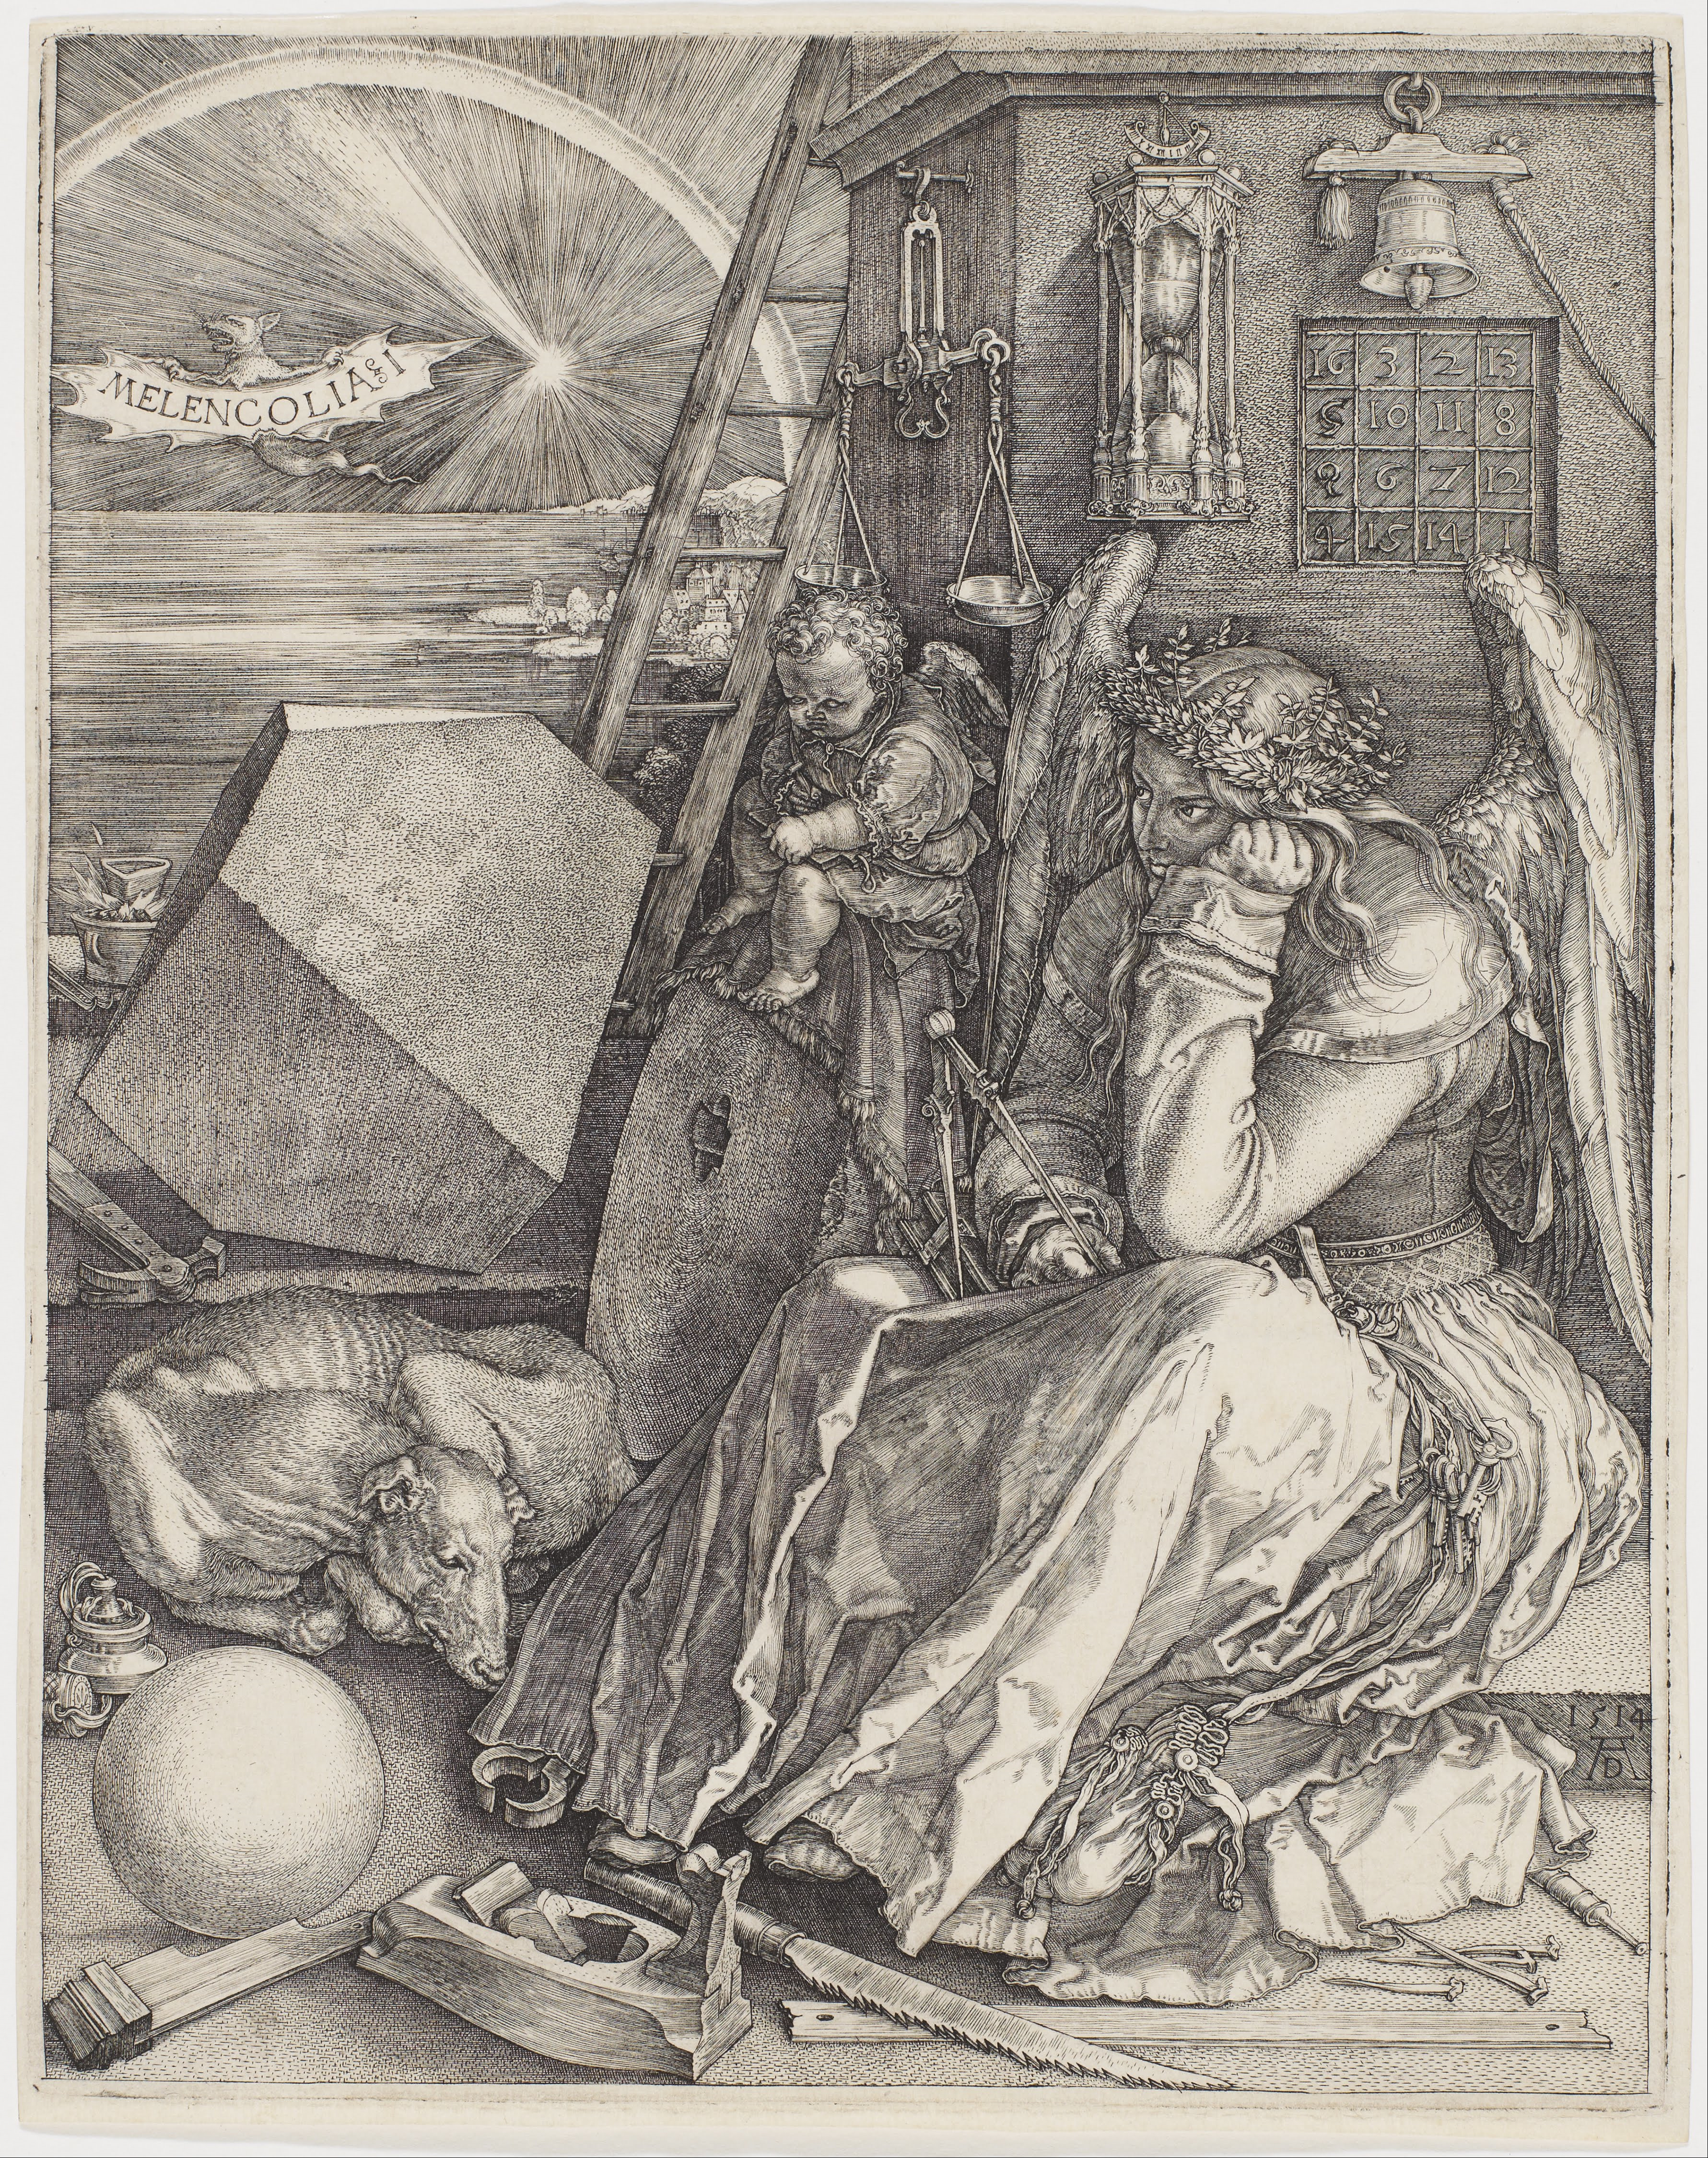
\includegraphics[width=0.45\columnwidth]{images/durer_melencolia.jpg}
    \caption{Albrecht Dürer, \textit{Melencolia I} (1514). Progressive cross-hatching for shading.}
    \label{fig:durer}
\end{figure}

I implemented this by adding more line layers as areas get darker. When the tone passes certain thresholds, new hatching directions are added, which creates that gradual darkening effect.

\section{Comparative Analysis}

\subsection{Visual Expressiveness}

Each NPR technique creates a different artistic style. Phong shading serves as the photorealistic baseline for technical accuracy. Toon shading produces a cartoon/anime cel look that works great for games and animation. Edge detection creates technical illustration style that emphasizes form clarity. Cross-hatching mimics classical engraving techniques and is perfect for artistic prints.

\subsection{Performance and Limitations}

All techniques run at 60+ FPS on my laptop GPU (NVIDIA GTX 1650) at 1920$\times$1080. I optimized edge detection with smart sampling (11 texture reads instead of 18), and cross-hatching is purely mathematical so it doesn't need any textures.

\textbf{Limitations}: Toon band boundaries can be jagged; edges may flicker with camera movement due to RGBA8 precision; hatching uses fixed angles that distort on curved surfaces.

\section{Technical Implementation}

I implemented 3 NPR techniques using a custom two-pass G-buffer pipeline for screen-space effects with geometric information access.

\subsection{Technique 1: Toon/Cel Shading}

\subsubsection{Algorithm}

Toon shading is the simplest NPR technique i implemented. It takes normal continuous lighting and quantizes it into discrete bands to create that cartoon-like appearance. I implemented this in view space to keep the math simpler:

{\footnotesize
\begin{algorithm}[H]
\caption{Toon Shading}
\begin{algorithmic}[1]
\State $\mathbf{N} \gets$ normalized view-space normal
\State $\mathbf{L} \gets$ normalized view-space light direction
\State $\text{diffuse\_raw} \gets \max(\mathbf{N} \cdot \mathbf{L}, 0)$
\State $\text{bands} \gets$ user-defined band count (2--8)
\State $\text{diffuse\_quantized} \gets \lfloor \text{diffuse\_raw} \times \text{bands} \rfloor / \text{bands}$
\State
\State $\mathbf{H} \gets$ normalize$(\mathbf{L} + \mathbf{V})$
\State $\text{specular\_raw} \gets \max(\mathbf{H} \cdot \mathbf{N}, 0)^{32}$
\State $\text{specular\_quantized} \gets$ step$(0.5, \text{specular\_raw})$
\State
\State $\text{color}_{\text{final}} \gets \text{baseColor} \times (0.25 + \text{diffuse\_quantized})$
\State \hspace{2.5em} $+ \text{lightColor} \times \text{specular\_quantized} \times 0.25$
\end{algorithmic}
\end{algorithm}
}

The floor function creates sharp boundaries between light and shadow, while the step function makes specular either fully on or off (no gradients). I added a slider to control band count from 2 to 8 so the cartoon effect can be adjusted.

\subsubsection{Implementation}

\begin{lstlisting}[language=C, caption=Toon Shading (GLSL excerpt)]
float bands = u_bands;
float diffuse = max(dot(N, L), 0.0);
float quantized = floor(diffuse * bands) / bands;

vec3 H = normalize(L + V);
float spec = pow(max(dot(N, H), 0.0), 32.0);
float specStep = step(0.5, spec);

vec3 result = baseColor * (0.25 + quantized) 
            + lightColor * specStep * 0.25;
\end{lstlisting}

\begin{figure}[!htb]
    \centering
    \begin{subfigure}{0.48\columnwidth}
        \includegraphics[width=\textwidth]{images/phong.png}
        \caption{Reference Phong}
    \end{subfigure}
    \hfill
    \begin{subfigure}{0.48\columnwidth}
        \includegraphics[width=\textwidth]{images/toon.png}
        \caption{Toon Shading (4 bands)}
    \end{subfigure}
    \caption{Comparison: Continuous vs. Quantized Lighting}
    \label{fig:toon_comparison}
\end{figure}

\subsection{Technique 2: Edge Detection}

\subsubsection{Algorithm}

For edge detection, i use Sobel operators on the G-buffer data. I detect edges from two different sources: depth discontinuities (where objects separate) and normal discontinuities (where surfaces crease). Combining both gives robust edge lines:

{\footnotesize
\begin{algorithm}[H]
\caption{Sobel-Based Edge Detection}
\begin{algorithmic}[1]
\State \textbf{Input:} G-buffer textures (normal+depth)
\State \textbf{Output:} Edge mask
\State
\For{each pixel $(x, y)$}
    \State Sample 3×3 neighborhood: $\{d_{-1,-1}, d_{-1,0}, \ldots, d_{1,1}\}$ (depth)
    \State Sample 3×3 neighborhood: $\{\mathbf{n}_{-1,-1}, \mathbf{n}_{-1,0}, \ldots, \mathbf{n}_{1,1}\}$ (normals)
    \State
    \State // Depth gradient (Sobel X/Y)
    \State $\nabla_x d \gets \sum_{i} d_i \times G_x[i]$
    \State $\nabla_y d \gets \sum_{i} d_i \times G_y[i]$
    \State $\text{edge}_{\text{depth}} \gets \sqrt{(\nabla_x d)^2 + (\nabla_y d)^2}$
    \State
    \State // Normal gradient
    \State $\nabla_x \mathbf{n} \gets \sum_{i} \mathbf{n}_i \times G_x[i]$
    \State $\nabla_y \mathbf{n} \gets \sum_{i} \mathbf{n}_i \times G_y[i]$
    \State $\text{edge}_{\text{normal}} \gets |\nabla_x \mathbf{n}| + |\nabla_y \mathbf{n}|$
    \State
    \State // Combined edge strength
    \State $\text{edge} \gets w_d \times \text{edge}_{\text{depth}} + w_n \times \text{edge}_{\text{normal}}$
    \State
    \If{$\text{edge} > \text{threshold}$}
        \State Output black line
    \Else
        \State Output original color
    \EndIf
\EndFor
\end{algorithmic}
\end{algorithm}
}

\textbf{Sobel Kernels}:
\begin{equation}
G_x = \begin{bmatrix}
-1 & 0 & +1 \\
-2 & 0 & +2 \\
-1 & 0 & +1
\end{bmatrix}, \quad
G_y = \begin{bmatrix}
-1 & -2 & -1 \\
0 & 0 & 0 \\
+1 & +2 & +1
\end{bmatrix}
\end{equation}

I used both depth and normals because depth edges catch the outer silhouette and overlapping objects, while normal edges detect surface details like creases and sharp corners. Combining them gives complete edge detection without extra geometry processing.

\begin{figure}[!htb]
    \centering
    \begin{subfigure}{0.48\columnwidth}
        \includegraphics[width=\textwidth]{images/edges_low.png}
        \caption{Low edge width (0.1)}
    \end{subfigure}
    \hfill
    \begin{subfigure}{0.48\columnwidth}
        \includegraphics[width=\textwidth]{images/edges_high.png}
        \caption{High edge width (0.6)}
    \end{subfigure}
    \caption{Edge Detection: Adjustable silhouette width using rim threshold}
    \label{fig:edges}
\end{figure}

\subsection{Technique 3: Cross-Hatching (My Extension)}

\subsubsection{How I Extended It: Progressive Layer System}

This is the technique that includes my extension. Instead of using pre-made textures like most hatching implementations do, i created a fully procedural system that generates lines mathematically. I designed it to follow Dürer's progressive layering approach where darker areas accumulate more and more line layers:

{\footnotesize
\begin{algorithm}[H]
\caption{Progressive Cross-Hatching}
\begin{algorithmic}[1]
\State $\text{tone} \gets 1 - \max(\mathbf{N} \cdot \mathbf{L}, 0)$ \Comment{0 = light, 1 = dark}
\State $\mathbf{uv} \gets \text{texture coordinates} \times \text{hatchScale}$
\State $\text{lineWidth} \gets 0.5$ \Comment{Relative to period}
\State
\State // Layer 1: Horizontal lines (0\textdegree)
\State $h_1 \gets$ step$(\text{lineWidth}, \text{fract}(\mathbf{uv}.y \times 15))$
\State
\State // Layer 2: Vertical lines (90\textdegree)
\State $h_2 \gets$ step$(\text{lineWidth}, \text{fract}(\mathbf{uv}.x \times 15))$
\State
\State // Layer 3: Diagonal lines (45$^\circ$)
\State $\mathbf{uv}_{\text{diag1}} \gets$ rotate$(\mathbf{uv}, 45^\circ)$
\State $h_3 \gets$ step$(\text{lineWidth}, \text{fract}(\mathbf{uv}_{\text{diag1}}.y \times 15))$
\State
\State // Layer 4: Counter-diagonal (-45$^\circ$)
\State $\mathbf{uv}_{\text{diag2}} \gets$ rotate$(\mathbf{uv}, -45^\circ)$
\State $h_4 \gets$ step$(\text{lineWidth}, \text{fract}(\mathbf{uv}_{\text{diag2}}.y \times 15))$
\State
\State // Layers 5 \& 6: Denser lines for very dark areas
\State $h_5 \gets$ step$(0.35, \text{fract}(\mathbf{uv}.y \times 22))$
\State $h_6 \gets$ step$(0.35, \text{fract}(\mathbf{uv}_{\text{diag1}}.y \times 22))$
\State
\State // Progressive accumulation
\State $\text{hatch} \gets 1.0$ \Comment{Start with white (no lines)}
\If{$\text{tone} > 0.12$}
    \State $\text{hatch} \gets h_1$ \Comment{Single direction}
\EndIf
\If{$\text{tone} > 0.30$}
    \State $\text{hatch} \gets \min(\text{hatch}, h_2)$ \Comment{Cross-hatch begins}
\EndIf
\If{$\text{tone} > 0.45$}
    \State $\text{hatch} \gets \min(\text{hatch}, h_3)$ \Comment{Add diagonal}
\EndIf
\If{$\text{tone} > 0.60$}
    \State $\text{hatch} \gets \min(\text{hatch}, h_4)$ \Comment{Full cross-hatch}
\EndIf
\If{$\text{tone} > 0.75$}
    \State $\text{hatch} \gets \min(\text{hatch}, h_5)$ \Comment{Increase density}
\EndIf
\If{$\text{tone} > 0.88$}
    \State $\text{hatch} \gets \min(\text{hatch}, h_6)$ \Comment{Maximum darkness}
\EndIf
\State
\State $\text{color}_{\text{lit}} \gets \text{baseColor} \times (0.3 + \mathbf{N} \cdot \mathbf{L} \times 0.7)$
\State $\text{color}_{\text{ink}} \gets \text{baseColor} \times 0.15$ \Comment{Dark ink}
\State \Return mix$(\text{color}_{\text{ink}}, \text{color}_{\text{lit}}, \text{hatch})$
\end{algorithmic}
\end{algorithm}
}



Each line layer is generated by rotating the UV coordinates and using \texttt{fract(uv.y * frequency)} to create periodic patterns. The \texttt{step} function turns this into black/white lines. I rotate the UVs by 0\textdegree, 45\textdegree, 90\textdegree, and -45\textdegree for different directions. The \texttt{min} operation accumulates layers - wherever lines overlap, the result gets darker.

I implemented 6 layers (most tutorials only do 2-3) with tone thresholds at 0.12, 0.30, 0.45, 0.60, 0.75, and 0.88. This gives smoother darkening like Dürer's engravings. Everything is procedural so there's no texture memory cost.


\begin{lstlisting}[language=C, caption=Cross-Hatching ]
float tone = 1.0 - clamp(dot(N, L), 0.0, 1.0);
vec2 uv = v_uv * u_hatchScale;

// Generate layers with rotation
float h1 = step(0.5, fract(uv.y * 15.0));
float h2 = step(0.5, fract(uv.x * 15.0));
vec2 d1 = mat2(0.707,-0.707,0.707,0.707) * uv;
float h3 = step(0.5, fract(d1.y * 15.0));
vec2 d2 = mat2(0.707,0.707,-0.707,0.707) * uv;
float h4 = step(0.5, fract(d2.y * 15.0));

// Accumulate based on tone
float hatch = 1.0;
if (tone > 0.12) hatch = h1;
if (tone > 0.30) hatch = min(hatch, h2);
if (tone > 0.45) hatch = min(hatch, h3);
if (tone > 0.60) hatch = min(hatch, h4);

vec3 lit = baseColor * (0.3 + ndotl * 0.7);
vec3 ink = baseColor * 0.15;
vec3 result = mix(ink, lit, hatch);
\end{lstlisting}

\begin{figure}[!htb]
    \centering
    \includegraphics[width=0.45\columnwidth]{images/cross_hatch.png}
    \caption{Cross-Hatching: Progressive layer accumulation inspired by Dürer's technique}
    \label{fig:hatching}
\end{figure}

\section{Conclusion}

This project taught me a lot about GPU programming and artistic rendering. I implemented 3 NPR techniques that all run at 60+ FPS on my GTX 1650.

The most interesting part was the cross-hatching extension. Instead of using textures like most implementations, i made it fully procedural with 6 layers. This means zero memory cost, infinite resolution, and real-time parameter control.

The G-buffer pipeline made it easy to experiment with different effects. The two-pass setup gives me screen-space edge detection while keeping geometric data for proper shading.

The hardest part was tuning the tone thresholds (0.12, 0.30, 0.45, 0.60, 0.75, 0.88) for the cross-hatching. I wanted gradual darkening like Dürer's engravings and i found suitable thresholds with trying.




% Bibliography (comment out if not using)
% \begin{thebibliography}{9}
% 
% \bibitem{praun2001tonal}
% Praun, E., Hoppe, H., Webb, M., \& Finkelstein, A. (2001).
% \textit{Real-time hatching}. 
% In Proceedings of the 28th annual conference on Computer graphics and interactive techniques (pp. 579-586).
% 
% \bibitem{gooch1998npr}
% Gooch, A., Gooch, B., Shirley, P., \& Cohen, E. (1998).
% \textit{A non-photorealistic lighting model for automatic technical illustration}.
% In Proceedings of the 25th annual conference on Computer graphics and interactive techniques (pp. 447-452).
% 
% \bibitem{lake2000stylized}
% Lake, A., Marshall, C., Harris, M., \& Blackstein, M. (2000).
% \textit{Stylized rendering techniques for scalable real-time 3D animation}.
% In Proceedings of the 1st international symposium on Non-photorealistic animation and rendering (pp. 13-20).
% 
% \end{thebibliography}

\end{document}